%
% 4_Goce.tex
%
% (c) 2020 Prof Dr Andreas Müller, Hochschule Rapperswil
%
% !TEX root = ../../buch.tex
% !TEX encoding = UTF-8
%
\section{GOCE
\label{planet:section:goce}}
\rhead{GOCE}

Die folgenden Angaben zur GOCE-Mission in diesem Abschnitt stammen von \cite{planet:goce}.

\begin{figure}[h]
    \centering
    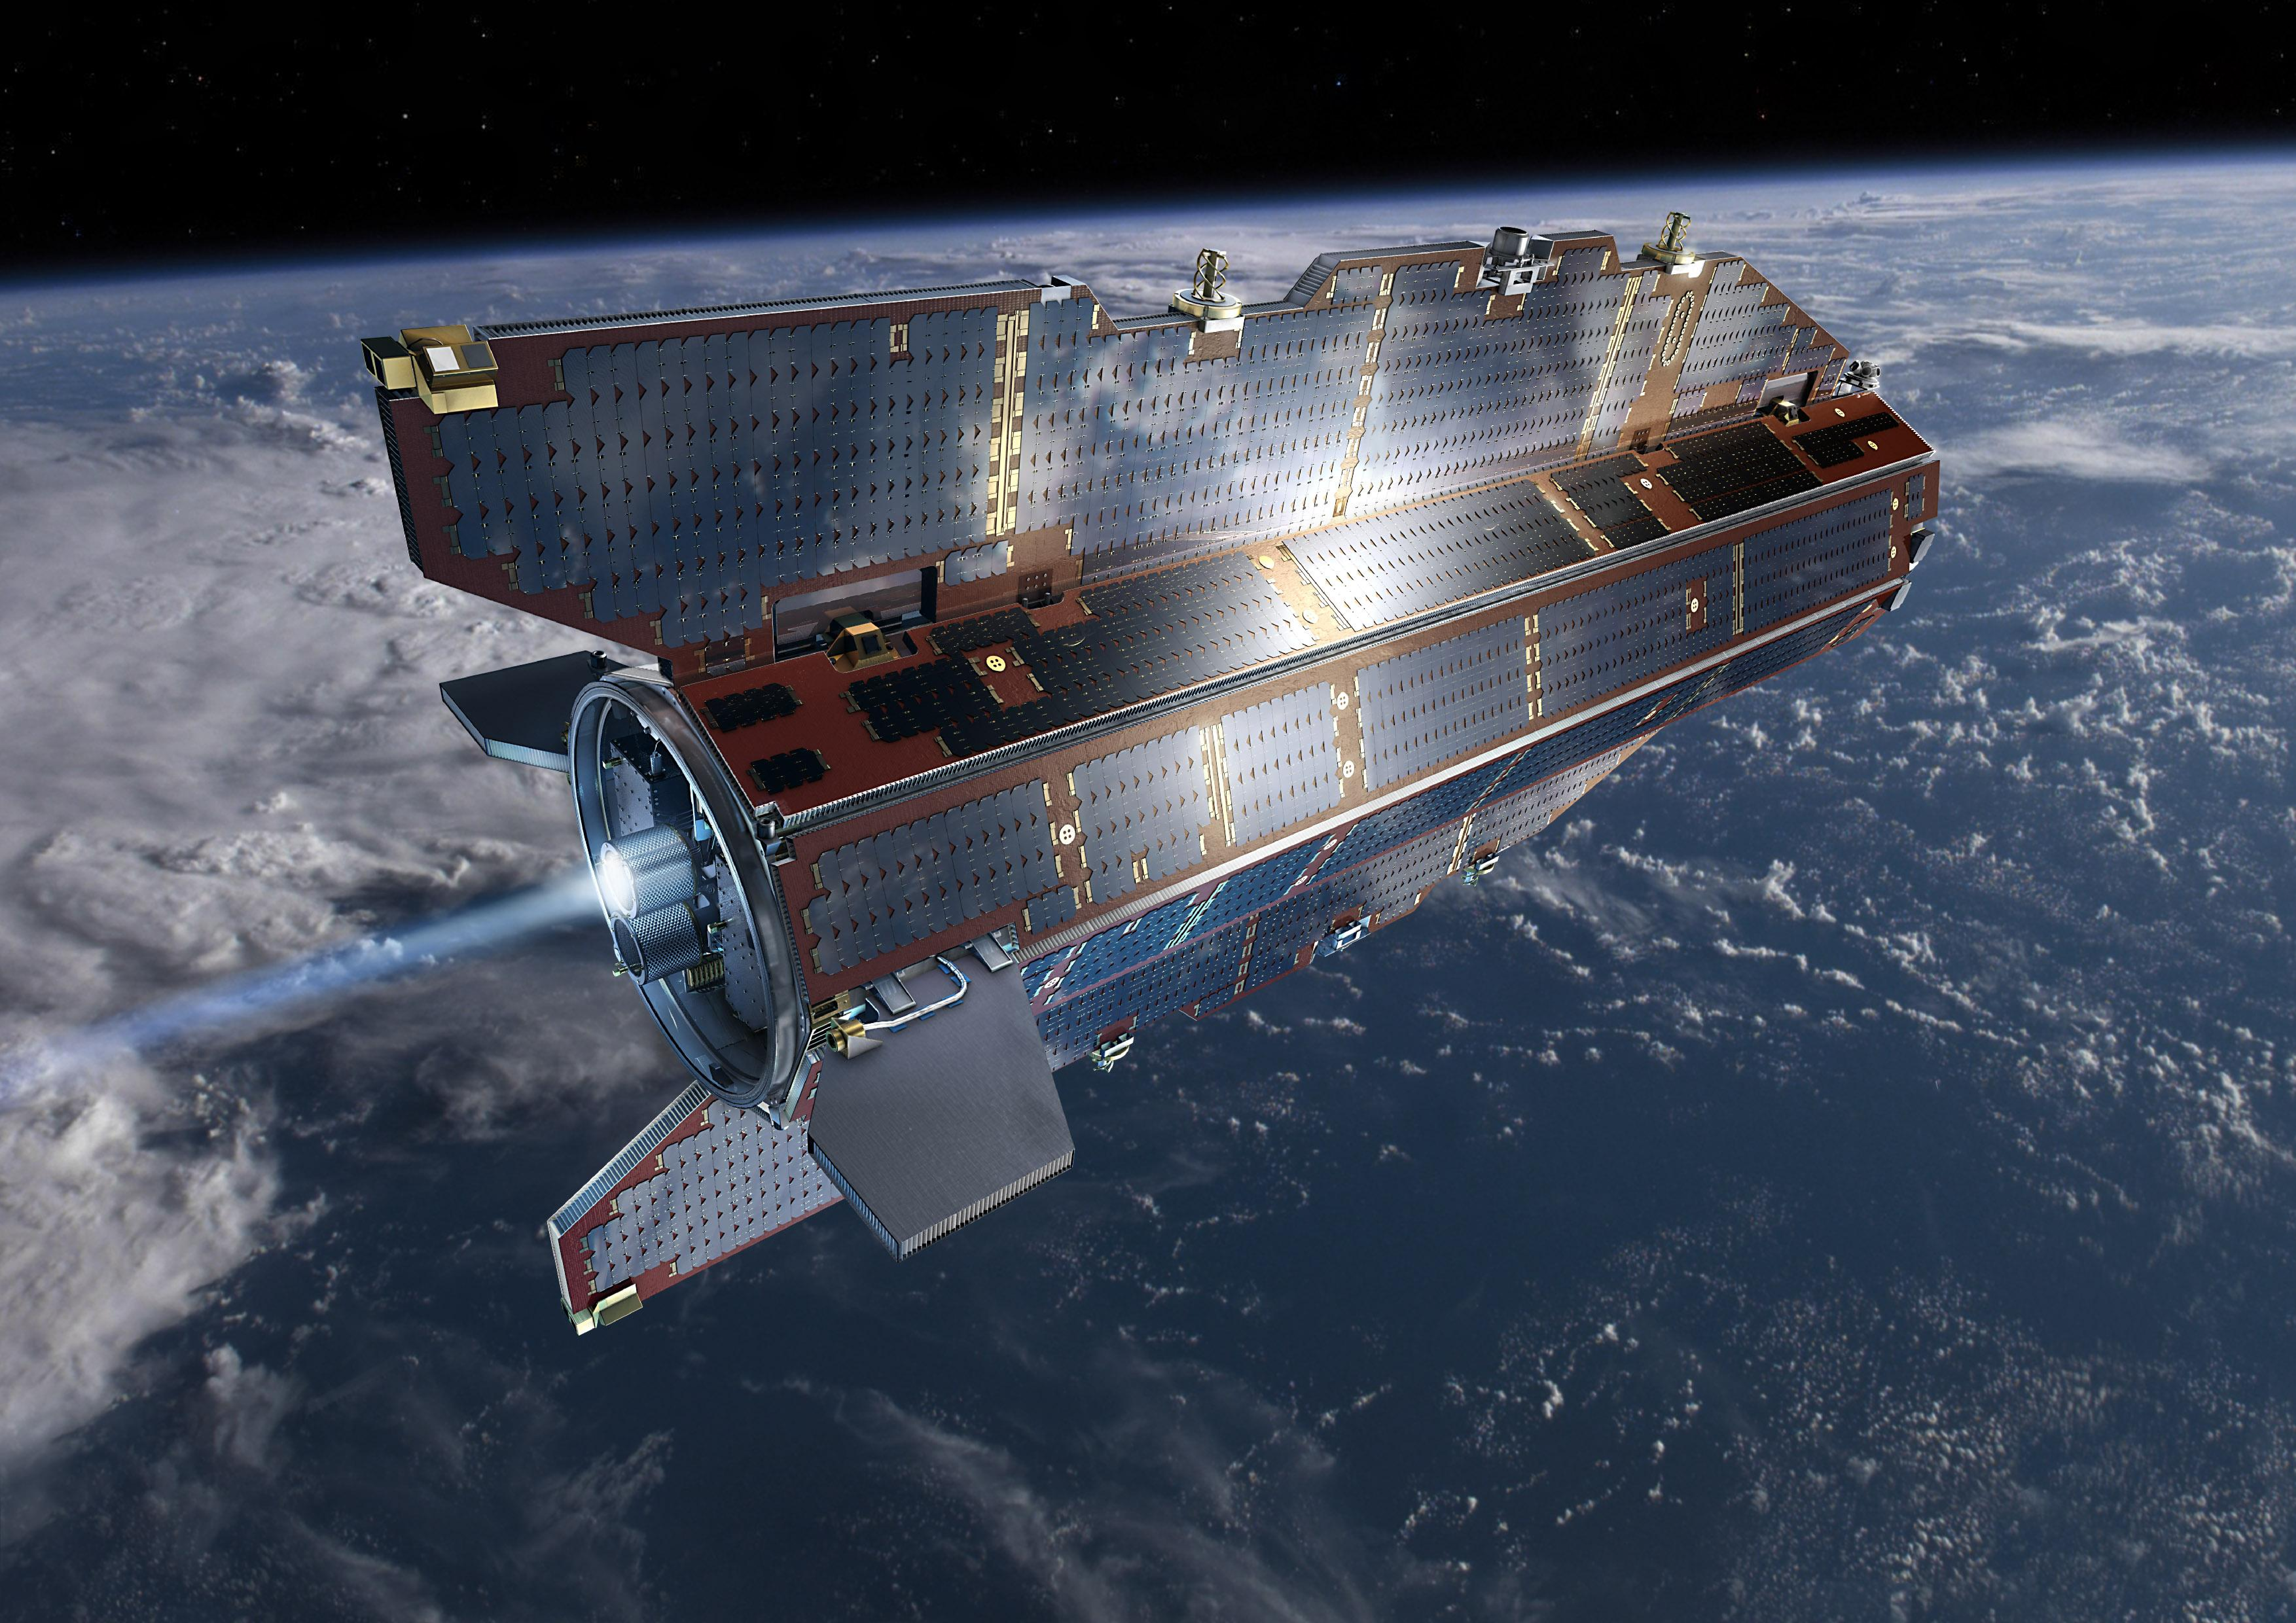
\includegraphics[width=\linewidth]{papers/planet/pictures/goce.pdf}
    \caption{Sattelit aus der GOCE Mission \cite{planet:gocepic}
        \label{planet:fig:goce}}
\end{figure}

Der Gravity Field and Steady-State Ocean Circulation Explorer (GOCE) ist ein Satellit, der im März 2009 von der Europäischen Weltraumorganisation ESA ins Weltall geschickt wurde.
GOCE umkreist die Erde in einer erdnahen Umlaufbahn von nur 260\,km Höhe, um das Schwerefeld der Erde mit bisher unerreichter Genauigkeit und räumlicher Auflösung zu erfassen.
Dafür nutzt GOCE einen Gradiometer unterstützt durch GPS um zusätzlich in Echtzeit die Navigation der Umlaufbahn aufzuzeichnen.

Das Gradiometer basiert auf drei Paaren von Beschleunigungssensoren.
Das Gradiometer misst den Gradienten der Gravitation, um eine sehr genaue Erfassung des Geoid der Erde zu erstellen, in \cref{planet:fig:geoid} zu sehen.
Dies gibt einen Einblick in die inneren Strukturen der Erde, sowie in die Strömungen in den Tiefen der Ozeane.
Die zweite Funktion des Gradiometers besteht darin, die Beschleunigung in Flugrichtung zu messen und den Schub von GOCE zu bestimmen, damit sich das Raumschiff nahezu im freien Fall befindet.

In der \cref{planet:fig:geoid} ist das Gravitationsfeld in den gelben Bereichen höher und in den blauen niedriger.
Aus dem \cref{planet:section:multipol} wird ersichtlich, was die Multipolentwicklung der Kugelform bedeutet, sie beschreibt die Abweichung von der perfekten Kugelform.
Die GOCE-Resultate werden daher mit den Multipolkoeffizienten geliefert.

\begin{figure}[h]
    \centering
    \includegraphics[width=\linewidth]{papers/planet/pictures/geoid.pdf}
    \caption{Darstellung des Gravitationsfelds der Erde \cite{planet:geoidpic}
        \label{planet:fig:geoid}}
\end{figure}


